\documentclass{IEEEtran}

\usepackage{tikz}
\usepackage{lipsum}

\usetikzlibrary{shapes.geometric, arrows}

\tikzset{
    objRectangle/.style={rectangle, minimum width=3cm, minimum height=1cm, text centered, draw=black, text width = 5cm},
    objRoundRectangle/.style={rectangle, rounded corners, minimum width=3cm, minimum height=1cm, text centered, draw=black, text width = 5cm},
    objRectangleMethods/.style={rectangle, minimum height=1cm, text centered, draw=black, text width = 3cm},
    arrow/.style={thick, ->, >=stealth}
}


\begin{document}

\lipsum[1]
\begin{figure*}[htbp]
    \centering
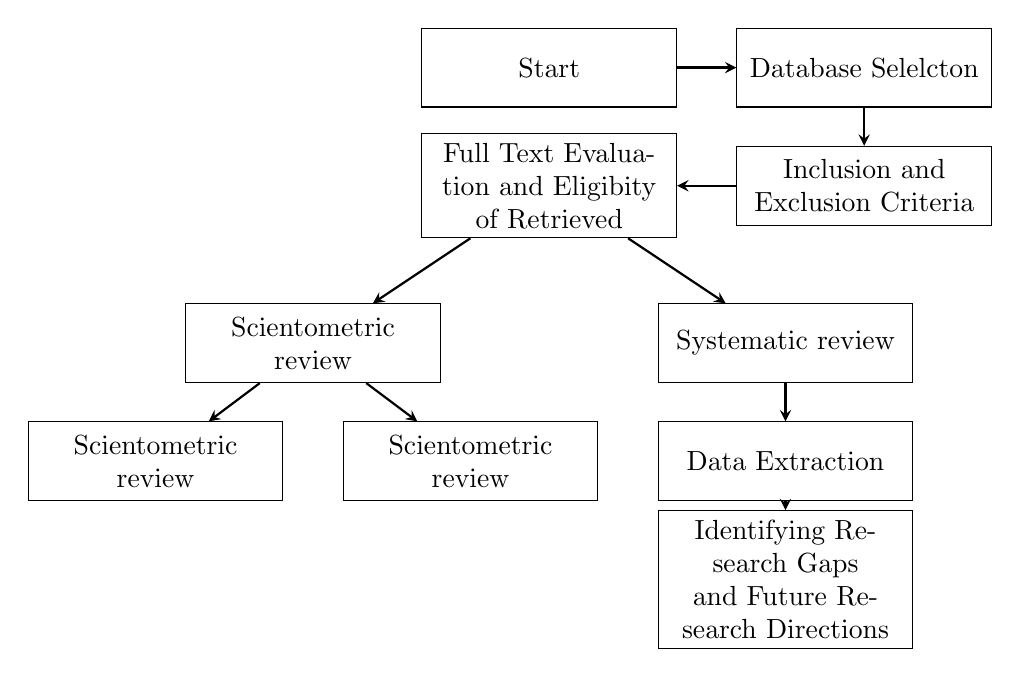
\begin{tikzpicture}[node distance=1.5cm]
    \node (001) [objRectangleMethods] {Start};
    \node (002) [objRectangleMethods, right of =001, xshift=2.5cm] {Database Selelcton};
    \node (003) [objRectangleMethods, below of=002] {Inclusion and Exclusion Criteria};
    \node (004) [objRectangleMethods, left of =003, xshift=-2.5cm] {Full Text Evaluation and Eligibity of Retrieved};

    \node (sci0) [objRectangleMethods, below of=004, xshift=-3cm, yshift=-0.5cm] {Scientometric review};
    \node (sci1a) [objRectangleMethods, below of=sci0, xshift=-2cm] {Scientometric review};
    \node (sci1b) [objRectangleMethods, below of=sci0, xshift=2cm] {Scientometric review};


    \node (sys0) [objRectangleMethods, below of=004, xshift=3cm, yshift=-0.5cm] {Systematic review};
    \node (sys1) [objRectangleMethods, below of=sys0] {Data Extraction };
    \node (sys2) [objRectangleMethods, below of=sys1] {Identifying Research Gaps and Future Research Directions};
    

    \draw[arrow] (001) -- (002);
    \draw[arrow] (002) -- (003);
    \draw[arrow] (003) -- (004);

    \draw[arrow] (004) -- (sci0);
    \draw[arrow] (sci0) -- (sci1a);
    \draw[arrow] (sci0) -- (sci1b);

    \draw[arrow] (004) -- (sys0);
    \draw[arrow] (sys0) -- (sys1);
    \draw[arrow] (sys1) -- (sys2);

\end{tikzpicture}
\caption{Outline of the Review Methodology}
\label{fig:flowchartMethod}
\end{figure*}

\lipsum[1]

\end{document}
